%%%%%%%%%%%%%%%%%%%%%%%%%%% COORDINATESYSTEMS
% COORDSYS (ORIGOCOORDINATENAME, WIDTH, HEIGHT)
% Draws a Coordinatesystem around ORIGOCOORDINATENAME with a width of WIDTH and a height of HEIGHT, 
% names the beginning and end of axes, southwest corner, northwest corner, 
\newcommand{\ThreeDimCoordSys}[4]{
\coordinate (XY#1) at ([xshift=#2 cm, yshift=#3 cm]#1);
\coordinate (-XY#1) at ([xshift=-#2 cm, yshift=-#3 cm]#1);
\coordinate (X#1) at ([xshift=#2 cm]#1);
\coordinate (-X#1) at ([xshift=-#2 cm]#1);
\coordinate (Y#1) at ([yshift=#3 cm]#1);
\coordinate (-Y#1) at ([yshift=-#3 cm]#1);
%\path (#1); \pgfgetlastxy{\XCoord}{\YCoord}; % Extracting coordinates of the Origin
%\pgfmathsetmacro{\XCoordcm}{\XCoord/28.4527}
%\pgfmathsetmacro{\YCoordcm}{\YCoord/28.4527}
%\coordinate (Z#1) at (\XCoordcm, \YCoordcm,#4);
%\coordinate (-Z#1) at (\XCoordcm, \YCoordcm,-#4);
%\draw [help lines, step=.5cm] (-XY#1) grid (XY#1);
\coordinate (Z#1) at ([shift=(\ThirdAxisAngle : #4*\ThirdAxisUnit cm)]#1);
\coordinate (-Z#1) at ([shift=(\ThirdAxisAngle : #4*\ThirdAxisUnit cm)]#1);
\draw[->, name path=XAxis#1] (#1)--(X#1);
\draw[->, name path=YAxis#1] (#1)--(Y#1);
\draw[->, name path=ZAxis#1] (#1)--(Z#1);
}

% \DistanceLabel{SS}{AS}{-45}{1}{pos=.5}{1}
\newcommand{\DistanceLabel}[6]{
\coordinate(#1horgony) at ([shift=(#3:#4)] #1);
\coordinate(#2horgony) at ([shift=(#3:#4)] #2);
\draw[thin, red, <->] (#1horgony)--(#2horgony) node[#5]{#6};
\draw[opacity=.4, black] (#1)--(#1horgony);
\draw[opacity=.4, black] (#2)--(#2horgony);
}

%Lorentz(OriginalOriginCoord, ResultingOriginCoord, SpeedNum, PointCoord, Label)
% 
\newcommand{\Lorentz}[5]{
\path (#1); \pgfgetlastxy{\XCoord}{\YCoord}; % Extracting coordinates of the Origin
\pgfmathsetmacro{\XOrigin}{\XCoord} % Saving X coordinate
\pgfmathsetmacro{\YOrigin}{\YCoord} % Saving Y coordinate
\path (#4); \pgfgetlastxy{\XCoord}{\YCoord}; % Extracting coordinates of the Point
\pgfmathsetmacro{\XEvent}{\XCoord} % Saving X coordinate
\pgfmathsetmacro{\YEvent}{\YCoord} % Saving Y coordinate
\pgfmathsetmacro{\XEventWRTOrigin}{\XEvent-\XOrigin} % Relativizing to the origin
\pgfmathsetmacro{\YEventWRTOrigin}{\YEvent-\YOrigin} % Relativizing to the origin
\pgfmathparse{XLorentz(#3,\XEventWRTOrigin,\YEventWRTOrigin)} % transforming x
\pgfmathsetmacro{\XEventTr}{\pgfmathresult} % save the result of x
\pgfmathparse{YLorentz(#3,\XEventWRTOrigin,\YEventWRTOrigin)} % transforming y
\pgfmathsetmacro{\YEventTr}{\pgfmathresult} % save the result of y
\node[world](#5) at (
[xshift=\XEventTr pt,
 yshift=\YEventTr pt] #2){};
}

\usetikzlibrary{calc}
\usetikzlibrary{intersections}
\newdimen\XCoord
\newdimen\YCoord

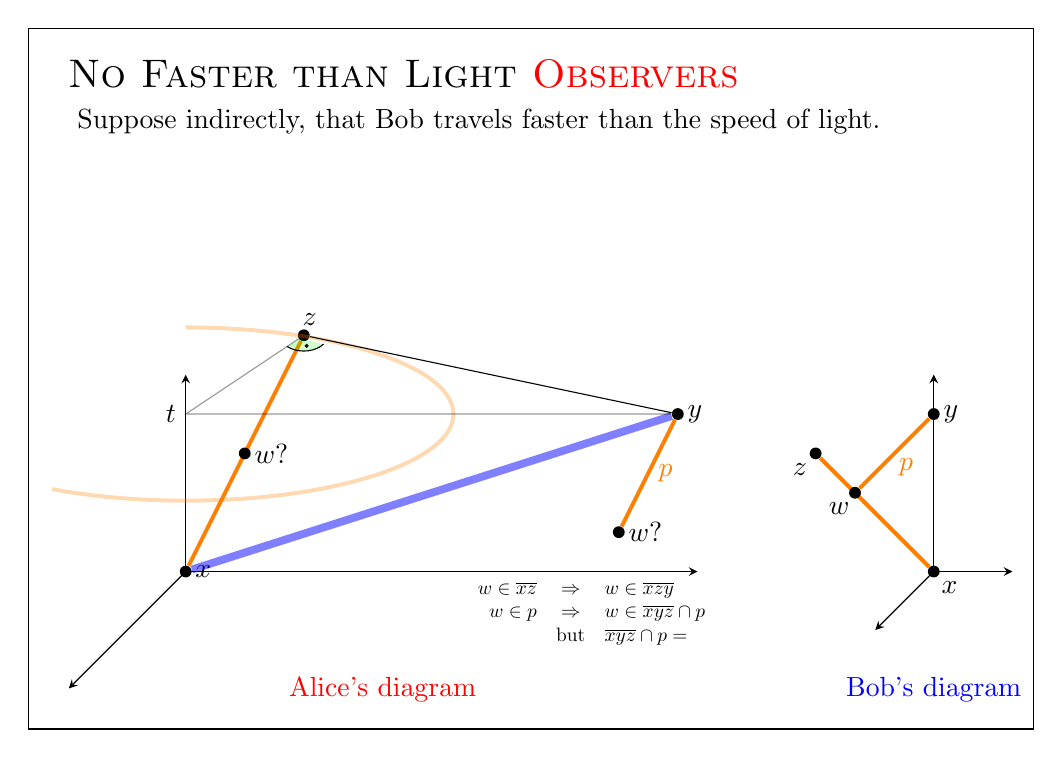
\begin{tikzpicture}[>=stealth, scale=1,
world/.style={inner sep=0, minimum size=.15cm, fill=black, circle},
worldline/.style={line width=1mm, rounded corners=1pt, opacity=.5},
axis/.style={->},
light/.style={orange, line width=.5mm},
]
\pgfmathdeclarefunction{XLorentz}{3}{\pgfmathparse{(#2 - #1*#3)/(sqrt(1-#1^2))}} % speed, spacecoord, timecoord
\pgfmathdeclarefunction{YLorentz}{3}{\pgfmathparse{(#3 - #1*#2)/(sqrt(1-#1^2))}} % speed, spacecoord, timecoord
\pgfmathsetmacro{\ThirdAxisAngle}{-135}
\pgfmathsetmacro{\ThirdAxisUnit}{.7}

%%%%%%%%%%%%%%%%%%%%%%%% DIA KEZDETE %%%%%%%%%%%%%%%%%%%%%%%%%%%

\node[anchor=north west, inner sep=0] at (0.5,8.5) {\textsc{\Large No Faster than Light \textcolor{red}{Observers}}}; %%%%%%% TITLE
%\node[anchor=north west, inner sep=0] at (0.5,8) {\textsc{\normalsize Role of Light}}; %%%%%%% SUBTITLE
\coordinate(jobbfelsosarok) at (12.77,8.9);
\draw%[white]  %%%%%%%%%%%% SIZE OF THE SLIDE
      (0,0) rectangle (jobbfelsosarok);
%%%%%%%%% TEXT %%%%%%%%%%%%%
\node[anchor=north west] at (0.5,8) {\begin{minipage}{11cm}
Suppose indirectly, that Bob travels faster than the speed of light. 
\end{minipage}
};
%%%%%%%%%%%%%%%%%%%%%%%% KOORDINÁTARENDSZEREK %%%%%%%%%%%%%%%%%%%%%%%%%%%
\coordinate(O1) at (2,2) {} {} {} {};
  \ThreeDimCoordSys{O1}{6.5}{2.5}{3}
\coordinate(O2) at (11.5,2) {} {} {} {} {};
  \ThreeDimCoordSys{O2}{1}{2.5}{1.5}

%%%%%%%%%%
%% SETTINGS %%
%%%%%%%%%%
\coordinate (BobStart) at (O1); % Fontos hogy átmenjen az Origón, különben rossz a lorentz transzformáció!!
\coordinate (BobEnd) at (1.25,6) {} {} {} {} {} {};

%%%%%%%%%%% Ezt lehetne macronak, speedszámítócuccnak
\path (BobStart); \pgfgetlastxy{\XCoord}{\YCoord}; % Extracting coordinates of the Origin
\pgfmathsetmacro{\XFirst}{\XCoord} % Saving X coordinate
\pgfmathsetmacro{\YFirst}{\YCoord} % Saving Y coordinate
\path (BobEnd); \pgfgetlastxy{\XCoord}{\YCoord}; % Extracting coordinates of the Point
\pgfmathsetmacro{\XSecond}{\XCoord} % Saving X coordinate
\pgfmathsetmacro{\YSecond}{\YCoord} % Saving Y coordinate
\pgfmathsetmacro{\SpeedBob}{(\XFirst-\XSecond)/(\YFirst-\YSecond)} % Relativizing to the origin
%%%%%%%%%%%%%%%%%%%%%%%%%%%%%%%%%%%

%\Lorentz{O1}{O1}{0}{BobStart}{BS}
%\Lorentz{O1}{O1}{0}{BobEnd}{BE}


\node[rotate=0, text=red, fill=white] at (4.5,0.5) {Alice's diagram};
\node[rotate=0, text=blue, fill=white] at (11.5,0.5) {Bob's diagram};


\node[world](x)at (O1) {};
\node[anchor=180] at (x) {$x$};
\node[world] (y) at (8.25,4) {};
\node[anchor=180] at (y) {$y$};
\draw[worldline, blue](x)--(y);

%\pause

\node[world] (z) at (3.5,5) {};
\node[anchor=250] at (z){$z$};
\draw[light] (x)--(z);

%\pause

\draw[light, opacity=.3] (2,5.1) arc (90:-120:3.4 and 1.1);
\coordinate(t) at ([yshift=2cm]O1);
\node[anchor=0] at (t){$t$};
\draw[opacity=.4] (y)--(t)--(z);
\draw  (y) edge (z);

\begin{scope}[shift={(0,0)}]
\clip (z)--(y)--(t)--(z);
\draw[fill=green, fill opacity=0.2, draw=black]  (z) ellipse (0.3 and 0.2);
\draw[fill=black] (3.5356,4.8666) circle (.5pt);
\end{scope}

%\pause

\node[world](x') at (O2){};
\node[anchor=135] at (x'){$x$};
\node[world] (y') at (11.5,4) {};
\node[anchor=180] at (y'){$y$};
\node[world] (z') at (10,3.5) {};
\node[anchor=45] at (z'){$z$};
\draw[light](x')--(z');

%\pause

\node[world] (w') at (10.5,3) {};
\node[anchor=45] at (w'){$w$};
\draw[light](w')--(y') node[midway, below right, inner sep=1]{$p$};

%\pause

\node[world] (w1) at (2.75,3.5) {};
\node[anchor=180] at (w1){$w?$};

%\pause

\node[world] (w2) at ([yshift=-1.5cm, xshift=-.75 cm]y) {};
\draw[light](w2)--(y)node[midway, right, inner sep=3]{$p$};
\node[anchor=180] at (w2){$w?$};

\node[anchor=north west, scale=.7] at (5.5,2) {$\begin{array}{rcl}
         w\in \overline{xz} & \Rightarrow & w \in \overline{xzy} 
%\pause
\\ w\in p &\Rightarrow & w \in \overline{xyz}  \cap  p
%\pause
     \\ &\textup{but} & \overline{xyz}  \cap  p= \varnothing
     \end{array}$};
\end{tikzpicture}